\section{Experiments and Results}

\begin{frame}{Testbed}
  \begin{figure}
    \centering
  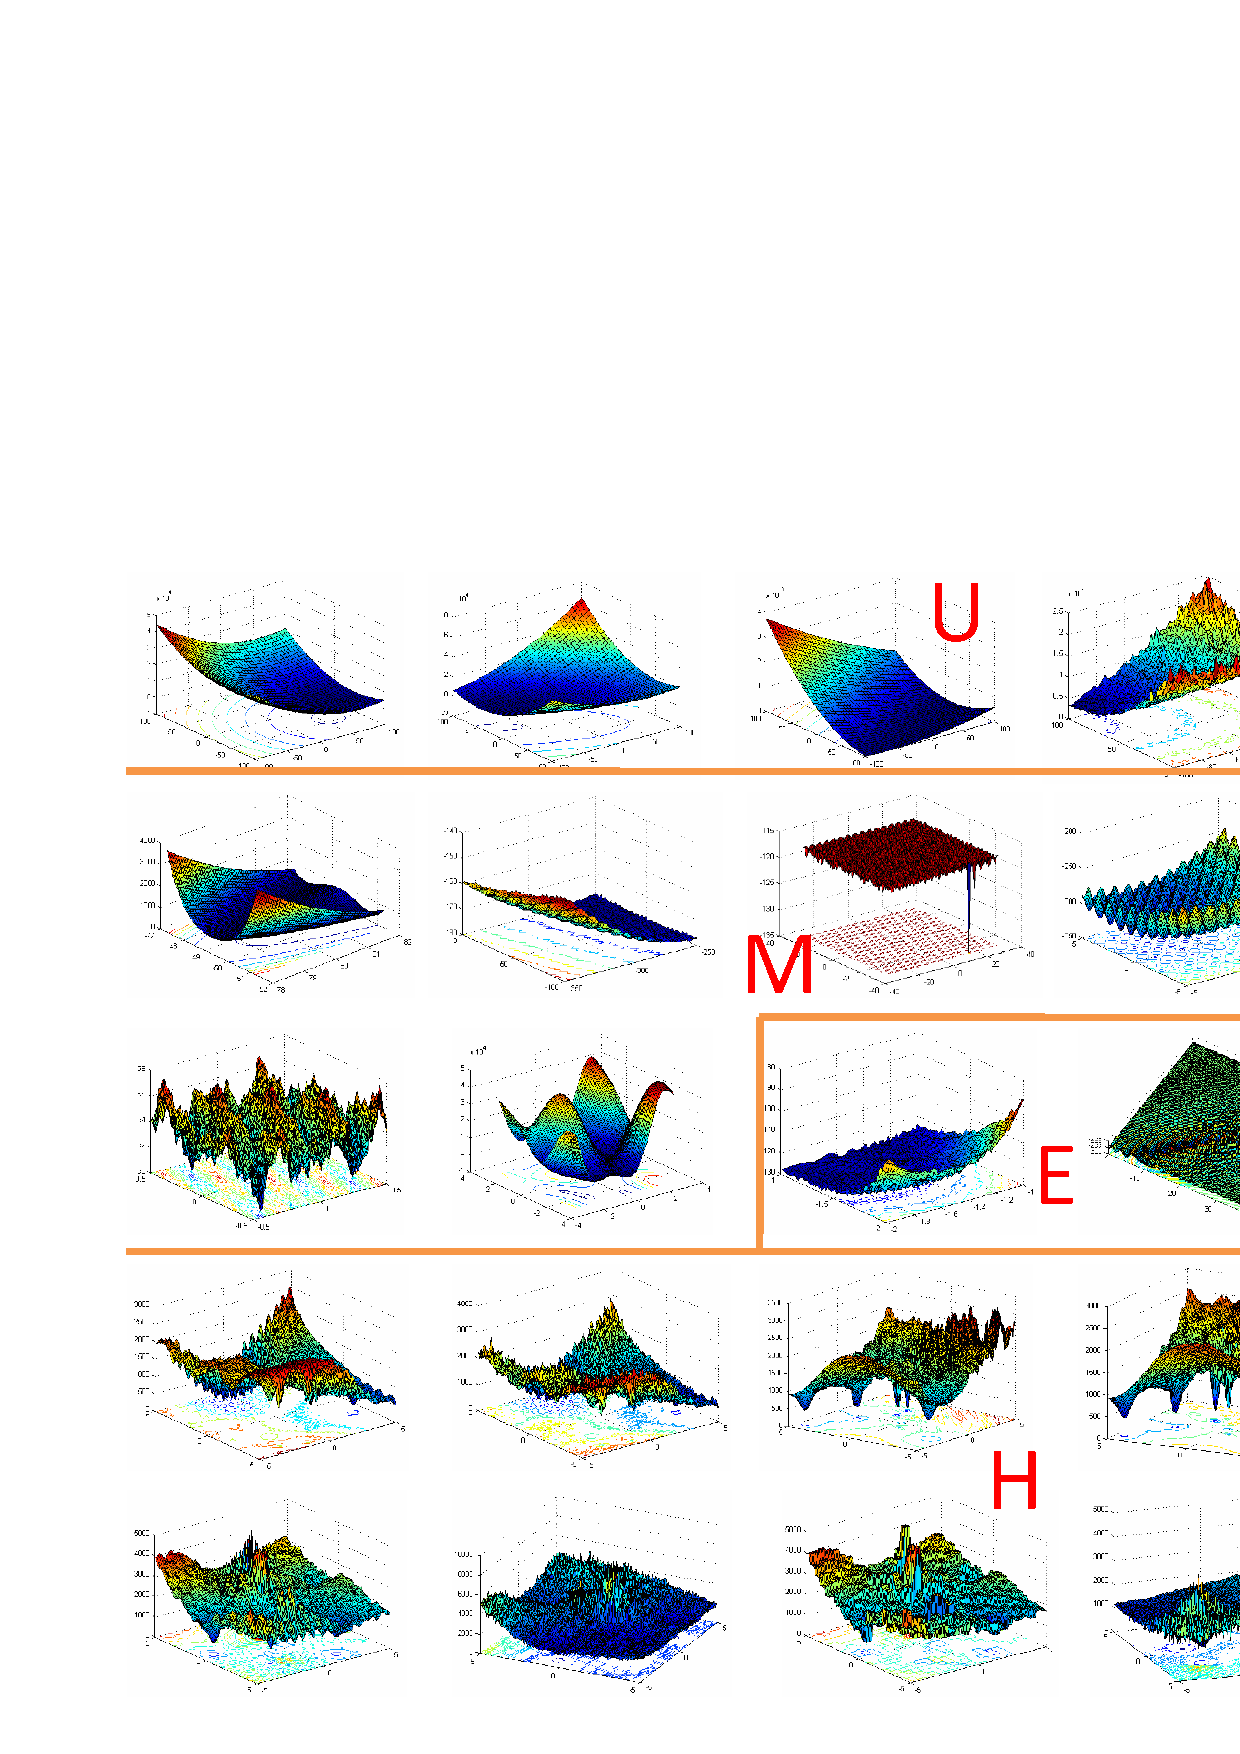
\includegraphics[bb= 43 16 783 584, clip, width =.8\textwidth]{benchmark}
\end{figure}
\end{frame}

\begin{frame}{Testbed}
  \begin{itemize}
    \item A set of benchmark proposed in CEC 2005 (Suganthan et al. 2005) 
      \vspace*{14pt}
    \item 25 problems are categorized into 4 kinds of problem that
      \begin{itemize}
        \item \alert{U}nimodal functions (1--5)
        \item \alert{M}ulti-modal functions (6--12)
        \item \alert{E}xpanded functions (13--14)
        \item \alert{H}ybrid composition functions (15--25)
      \end{itemize}
      \vspace*{14pt}
    \item Benchmark criteria
      \begin{itemize}
        \item The best accuracy after $10^5$ function evaluations
      \end{itemize}
  \end{itemize}
\end{frame}


\begin{frame}{Experiments Design}
  \begin{itemize}
    \item Comparison for robustness is performed
      \vspace*{14pt}
    \item 2 comparisons
      \begin{enumerate}
        \item Comparing to original CMA-ES 
        \item Comparing to rECGA + SoD
      \end{enumerate}
      \vspace*{14pt}
    \item The judging criteria
      \begin{itemize}
        \item Each problem runs 25 times.
        \item The best, median, worst solutions of each run are collected.
      \end{itemize}
  \end{itemize}
\end{frame}

\begin{frame}{Comparison to Original CMA-ES}
  \begin{itemize}
    \item For all instance of CMA-ES, $\lambda = 20$ and $\sigma$ is
      initial to $1$.
    \item For each pull option, the 1st layer CMA-ES executes for $30$
      iterations.
    \item The population size is set to be $450$ and $k = 15$ for
      MAB based CMA-ES.
  \end{itemize}
  \begin{columns}
    \footnotesize
    \begin{column}{0.5\textwidth}
\begin{table}[h]
\begin{tabular}{|c|c|c|}
\hline
      & \begin{tabular}[c]{@{}c@{}}Original\\ CMA-ES\end{tabular} & \begin{tabular}[c]{@{}c@{}}MAB-basd\\ CMA-ES\end{tabular} \\ \hline
U     & --                                                       & --              \\ \hline
M     & --                                                       & 1               \\ \hline
E     & --                                                       & 2               \\ \hline
H     & --                                                       & 6               \\ \hline
Total & --                                                       & 9               \\ \hline
\end{tabular}
\caption{Comparison of best run}
\end{table}
      
    \end{column}
\begin{column}{0.5\textwidth}
\begin{table}[h]
\begin{tabular}{|c|c|c|}
\hline
      & \begin{tabular}[c]{@{}c@{}}Original\\ CMA-ES\end{tabular} & \begin{tabular}[c]{@{}c@{}}MAB-basd\\ CMA-ES\end{tabular} \\ \hline
U     & --
& --                                                         \\ \hline
M     & --
& 3                                                         \\ \hline
E     & --                                                       & 2                                                         \\ \hline
H     & 1
& 9                                                         \\ \hline
Total & 1                                                        &
14                                                        \\ \hline
\end{tabular}
\caption{Comparison of median run}
\end{table}
\end{column}
  \end{columns}

\end{frame}
\begin{frame}{Comparison to rECGA + SoD}
  \begin{itemize}
    \item Same settings as SoD paper
  \end{itemize}
\begin{columns}
\begin{column}{0.5\textwidth}
\begin{table}[h]
\begin{tabular}{|c|c|c|}
\hline
      & \begin{tabular}[c]{@{}c@{}}rECGA+\\ SoD\end{tabular} & \begin{tabular}[c]{@{}c@{}}MAB-basd\\ CMA-ES\end{tabular} \\ \hline
U     & --
& 5                                                    \\ \hline
M     & 1                                                         &
5                                                    \\ \hline
E     & 2                                                         &
--                                                    \\ \hline
H     & 4                                                         & 4                                                    \\ \hline
Total & 7                                                        &
14                                                   \\ \hline
\end{tabular}
\caption{Comparison of best run}
\end{table}
\end{column}
\begin{column}{0.5\textwidth}
 \begin{table}[h]
\begin{tabular}{|c|c|c|}
\hline
      & \begin{tabular}[c]{@{}c@{}}rECGA+\\ SoD\end{tabular} & \begin{tabular}[c]{@{}c@{}}MAB-basd\\ CMA-ES\end{tabular} \\ \hline
U     & --
& 5                                                    \\ \hline
M     & 1
& 5                                                    \\ \hline
E     & 2
& --                                                    \\ \hline
H     & 2
& 8                                                    \\ \hline
Total & 5
& 18                                                    \\ \hline
\end{tabular}
\caption{Comparison of median run}
\end{table} 
\end{column}

\end{columns}

\end{frame}
\begin{frame}{Discussion}
 
  \begin{itemize}
    \item Strength
      \begin{itemize}
        \item Higher median values in 18 problems comparing to rECGA+SoD.
        \item Higher median values in all multimodel problems except
          problem 22 compaing to CMA-ES
      \end{itemize}
      \vspace*{14pt}
    \item Weakness
      \begin{itemize}
        \item Reach no global optimum in problems addressed by a dence
          distribution of local optima.
        \item Too complicated for simple problem.
      \end{itemize}
      \vspace*{14pt}
    \item Improvement
      \begin{itemize}
        \item Ruggedness
        \item Non-convex
      \end{itemize}

  \end{itemize}

\end{frame}
%\begin{frame}{Comparison}
%  \begin{itemize}
%    \item For original CMA-ES, the $\lambda$ is set to 20 and $\sigma$
%      is initialized to 1.
%    \item For 2-layer CMA-ES, the $\lambda$ and $\sigma$ is as above.
%    \item For 2-layer CMA-ES, the initial population size is set to 450
%      and inner CMA-ES executes for $1000$ generations.
%  \end{itemize}
%  \begin{columns}
%    \footnotesize
%    \begin{column}{0.5\textwidth}
%      \begin{table}[h]
%        \begin{tabular}{|c|c|c|}
%          \hline
%          & CMA-ES & 2-Layer CMA-ES \\ \hline
%          U & --     & --             \\ \hline
%          B & --     & 1              \\ \hline
%          E & --     & 2              \\ \hline
%          H & 2      & 4              \\ \hline
%          Total & 2 & 7 \\\hline
%        \end{tabular}
%        \caption{Best accuracy comparison}
%      \end{table}
%    \end{column}
%    \begin{column}{0.5\textwidth}
%      \begin{table}[h]
%        \begin{tabular}{|c|c|c|}
%          \hline
%          & CMA-ES & 2-Layer CMA-ES \\ \hline
%          U     & 1      & --             \\ \hline
%          B     & 2      & 1              \\ \hline
%          E     & --     & 2              \\ \hline
%          H     & 3      & 5              \\ \hline
%          Total & 6      & 8              \\ \hline
%        \end{tabular}
%        \caption{Median accuracy comparison}
%      \end{table}
%    \end{column}
%
%  \end{columns}
%\end{frame}
%
%\begin{frame}{Comparison}
%  \begin{itemize}
%    \item 2-layer CMA-ES is set as above.
%    \item MAB-based CMA-ES sets $t$ of inner CMA-ES to be 30 and $t$ of
%      outer CMA-ES to be 1. Other settings are identical to 2-layer CMA-ES.\
%  \end{itemize}
%  \begin{columns}
%    \footnotesize
%    \begin{column}{0.5\textwidth}
%\begin{table}[h]
%\begin{tabular}{|c|c|c|}
%\hline
%      & \begin{tabular}[c]{@{}c@{}}2-Layer\\ CMA-ES\end{tabular} & \begin{tabular}[c]{@{}c@{}}MAB-basd\\ CMA-ES\end{tabular} \\ \hline
%U     & --                                                       & --              \\ \hline
%B     & --                                                       & --              \\ \hline
%E     & 1                                                        & 1               \\ \hline
%H     & 2                                                        & 3               \\ \hline
%Total & 3                                                        & 4               \\ \hline
%\end{tabular}
%\caption{Best accuracy comparison}
%\end{table}
%      
%    \end{column}
%\begin{column}{0.5\textwidth}
%\begin{table}[h]
%\begin{tabular}{|c|c|c|}
%\hline
%      & \begin{tabular}[c]{@{}c@{}}2-Layer\\ CMA-ES\end{tabular} & \begin{tabular}[c]{@{}c@{}}MAB-basd\\ CMA-ES\end{tabular} \\ \hline
%U     & --                                                       & 1                                                         \\ \hline
%B     & --                                                       & 4                                                         \\ \hline
%E     & --                                                       & 2                                                         \\ \hline
%H     & 2                                                        & 8                                                         \\ \hline
%Total & 2                                                        & 15                                                        \\ \hline
%\end{tabular}
%\caption{Median accuracy comparison}
%\end{table}
%\end{column}
%  \end{columns}
%
%\end{frame}

